\documentclass[12pt, titlepage]{article}

\usepackage{booktabs}
\usepackage{tabularx}
\usepackage{hyperref}
\usepackage{graphicx}
\usepackage{float}
\hypersetup{
    colorlinks,
    citecolor=blue,
    filecolor=black,
    linkcolor=red,
    urlcolor=blue
}
\usepackage[round]{natbib}

%% Comments

\usepackage{color}

\newif\ifcomments\commentstrue %displays comments
%\newif\ifcomments\commentsfalse %so that comments do not display

\ifcomments
\newcommand{\authornote}[3]{\textcolor{#1}{[#3 ---#2]}}
\newcommand{\todo}[1]{\textcolor{red}{[TODO: #1]}}
\else
\newcommand{\authornote}[3]{}
\newcommand{\todo}[1]{}
\fi

\newcommand{\wss}[1]{\authornote{blue}{SS}{#1}} 
\newcommand{\plt}[1]{\authornote{magenta}{TPLT}{#1}} %For explanation of the template
\newcommand{\an}[1]{\authornote{cyan}{Author}{#1}}

%% Common Parts

\newcommand{\progname}{OCRacle} % PUT YOUR PROGRAM NAME HERE
\newcommand{\authname}{Phillip Tran} % AUTHOR NAMES                  

\usepackage{hyperref}
    \hypersetup{colorlinks=true, linkcolor=blue, citecolor=blue, filecolor=blue,
                urlcolor=blue, unicode=false}
    \urlstyle{same}
                                


\begin{document}

\title{System Verification and Validation Plan for \progname{}} 
\author{\authname}
\date{\today}
	
\maketitle

\pagenumbering{roman}

\section*{Revision History}

\begin{tabularx}{\textwidth}{p{4cm}p{2cm}X}
\toprule {\bf Date} & {\bf Version} & {\bf Notes}\\
\midrule
February 20, 2025 & 1.0 & Initial Creation\\
April 1, 2025 & 2.0 & Added unit tests\\
April 5, 2025 & 2.1 & Addressed feedback from Dr. Spencer Smith\\
April 7, 2025 & 2.2 & Addressed Feedback from Hussein Saad\\
\bottomrule
\end{tabularx}

% ~\\
% \wss{The intention of the VnV plan is to increase confidence in the software.
% However, this does not mean listing every verification and validation technique
% that has ever been devised.  The VnV plan should also be a \textbf{feasible}
% plan. Execution of the plan should be possible with the time and team available.
% If the full plan cannot be completed during the time available, it can either be
% modified to ``fake it'', or a better solution is to add a section describing
% what work has been completed and what work is still planned for the future.}

% \wss{The VnV plan is typically started after the requirements stage, but before
% the design stage.  This means that the sections related to unit testing cannot
% initially be completed.  The sections will be filled in after the design stage
% is complete.  the final version of the VnV plan should have all sections filled
% in.}

\newpage

\tableofcontents

\listoftables
% \wss{Remove this section if it isn't needed}

% \listoffigures
% \wss{Remove this section if it isn't needed}

\newpage

\section{Symbols, Abbreviations, and Acronyms}

\renewcommand{\arraystretch}{1.2}
\begin{tabular}{l l} 
  \toprule		
  \textbf{symbol} & \textbf{description}\\
  \midrule 
  T & Test\\
  OCR & Optical Character Recognition\\
  OAR & Optical Alphabet Recognition, the predecessor to this program\\
  SRS & Software Requirements Specification\\
  VnV & Verification and Validation\\
  MG & Module Guide\\
  MIS & Module Interface Specification\\
  PEP 8 & Python Enhancement Proposal 8, the Python style guide\\
  GHA & GitHub Actions\\
  \bottomrule
\end{tabular}\\

% \wss{symbols, abbreviations, or acronyms --- you can simply reference the SRS
%   \cite{SRS} tables, if appropriate}

% \wss{Remove this section if it isn't needed}

\newpage

\pagenumbering{arabic}

This document outlines the verification and validation plan for the \progname{}
program. This document will outline the testing procedures that will be used to
ensure that the software meets the requirements outlined in the SRS document \citep{SRS}.

\section{General Information}

\subsection{Summary}

The \progname{} program is being tested. \progname{} is an OCR program that classifies
a single handwritten uppercase Latin alphabet character in an image. The project
provides a trained model to complete this task as well as a user interface to
feed an image into the model and display the model's predicted character.

% \wss{Say what software is being tested.  Give its name and a brief overview of
%   its general functions.}

\subsection{Objectives}

The main objective of this project is to build confidence in the software
correctness. This will be done by testing the software to ensure that it meets
the requirements outlined in the SRS document. This includes testing the accuracy
of the software as compared to the OAR predecessor. Validation of the software's
maintainability will also be conducted.

For the purposes of this project, the validation of the program's usability
will not be heavily tested. This is because the program's user interface will be
kept as simple as possible to focus on the OCR functionality.

The project may rely on external libraries for image manipulation or matrix
operations. The validation of these libraries will not be tested.

% \wss{State what is intended to be accomplished.  The objective will be around
%   the qualities that are most important for your project.  You might have
%   something like: ``build confidence in the software correctness,''
%   ``demonstrate adequate usability.'' etc.  You won't list all of the qualities,
%   just those that are most important.}

% \wss{You should also list the objectives that are out of scope.  You don't have 
% the resources to do everything, so what will you be leaving out.  For instance, 
% if you are not going to verify the quality of usability, state this.  It is also 
% worthwhile to justify why the objectives are left out.}

% \wss{The objectives are important because they highlight that you are aware of 
% limitations in your resources for verification and validation.  You can't do everything, 
% so what are you going to prioritize?  As an example, if your system depends on an 
% external library, you can explicitly state that you will assume that external library 
% has already been verified by its implementation team.}

\subsection{Challenge Level and Extras}

The challenge level for this project is general. Although this project has been
done before, implementing the software with higher accuracy than the previous
implementation is a challenge.

For the extra task, I will be including a user manual. This will help users
understand how to use the program and what to expect from it.

% \wss{State the challenge level (advanced, general, basic) for your project.
% Your challenge level should exactly match what is included in your problem
% statement.  This should be the challenge level agreed on between you and the
% course instructor.  You can use a pull request to update your challenge level
% (in TeamComposition.csv or Repos.csv) if your plan changes as a result of the
% VnV planning exercise.}

% \wss{Summarize the extras (if any) that were tackled by this project.  Extras
% can include usability testing, code walkthroughs, user documentation, formal
% proof, GenderMag personas, Design Thinking, etc.  Extras should have already
% been approved by the course instructor as included in your problem statement.
% You can use a pull request to update your extras (in TeamComposition.csv or
% Repos.csv) if your plan changes as a result of the VnV planning exercise.}

\subsection{Relevant Documentation}

% \wss{Reference relevant documentation.  This will definitely include your SRS
%   and your other project documents (design documents, like MG, MIS, etc).  You
%   can include these even before they are written, since by the time the project
%   is done, they will be written.  You can create BibTeX entries for your
%   documents and within those entries include a hyperlink to the documents.}

  \begin{itemize}
    \item SRS Document \citep{SRS}: Outlines the requirements for the \progname{}
    program. This VnV plan will be based on the requirements outlined in this
    document.
    \item MG Document \citep{MG}: Outlines the modules that compose the \progname{} program.
    The VnV plan will be based on the modules outlined in this document.
    \item MIS Document \citep{MIS}: Outlines the interfaces of the modules that compose the
    \progname{} program. The VnV plan will be based on the interfaces outlined in
    this document.
  \end{itemize}

% \wss{Don't just list the other documents.  You should explain why they are relevant and 
% how they relate to your VnV efforts.}

\section{Plan}

This section outlines the multiple stages of the verification and validation
process. First, the VnV team will be introduced. Then the verification plans for
the SRS, design, VnV plan, and implementation will be outlined. Finally, a brief
overview of automated testing and verification tools will be provided. 

% \wss{Introduce this section.  You can provide a roadmap of the sections to
%   come.}

\subsection{Verification and Validation Team}

% \wss{Your teammates.  Maybe your supervisor.
%   You should do more than list names.  You should say what each person's role is
%   for the project's verification.  A table is a good way to summarize this information.}

The following personnel will be involved in the verification and validation of
the \progname{} program:

\begin{itemize}
  \item \authname: The author of the program. Will be responsible for the
  verification and validation of the \progname{} program. This includes the creation
  of the VnV plan, the implementation of the tests, and the analysis of the
  results.
  \item Dr.~Spencer Smith: The instructor. Will be responsible for the
  verification and validation of the \progname{} program. This includes the review
  of the VnV plan, the review of the tests, and the review of the results.
  \item Hussein Saad: The domain expert. Will be responsible for the
  verification and validation of the \progname{} program. This includes the review
  of the VnV plan, the review of the tests, and the review of the results.
\end{itemize}

\subsection{SRS Verification Plan}

To validate the SRS, the domain expert and instructor have been assigned a
GitHub issues to review the document. The author will be responsible for
addressing any comments made by the reviewers. As the project progresses
the SRS document may be modified, and the reviewers will be assigned a new
GitHub issue to review the changes.

To ensure that the SRS document is complete, correct, and consistent, the
reviewers can rely on the SRS checklist \citep{SRSChecklist}.

\subsection{Design Verification Plan}

The design of the \progname{} program will be verified by the domain expert and
instructor using the MG checklist \citep{MGChecklist} and MIS checklist \citep{MISChecklist}.

Reviewers will focus on ensuring that the modules and interfaces are correctly
defined for the \progname{} program given the requirements outlined in the SRS
document.


% \wss{Plans for design verification}

% \wss{The review will include reviews by your classmates}

% \wss{Create a checklists?}

\subsection{Verification and Validation Plan Verification Plan}

The VnV plan will be reviewed by the domain expert and instructor using the 
VnV plan checklist \citep{VnVChecklist}. The author will be responsible for
addressing any comments made by the reviewers. As the project progresses the
VnV plan may be modified, and the reviewers will be assigned a new GitHub issue
to review the changes.

Reviewers will focus on ensuring that test cases adequately cover any edge cases
and are representative of the requirements outlined in the SRS document.

% \wss{The verification and validation plan is an artifact that should also be
% verified.  Techniques for this include review and mutation testing.}

% \wss{The review will include reviews by your classmates}

% \wss{Create a checklists?}

\subsection{Implementation Verification Plan}

As described in Section \ref{sec:AutomatedTesting}, the \progname{} program will
be tested using an automated test suite. Code quality and static type checking
will also be enforced using automated tools. To ensure that these automated
tests are correct, the VnV team will review the tests and the test results. The
VnV team will also review the code quality and static type checking results.

Manual testing in the form of code walkthroughs will also be used to ensure that
the code is achieving the desired functionality. This will be the primary
responsibility of the author, with the domain expert and instructor providing
feedback of the code walkthroughs to ensure that the code is correct.

% \wss{You should at least point to the tests listed in this document and the unit
%   testing plan.}

% \wss{In this section you would also give any details of any plans for static
%   verification of the implementation.  Potential techniques include code
%   walkthroughs, code inspection, static analyzers, etc.}

% \wss{The final class presentation in CAS 741 could be used as a code
% walkthrough.  There is also a possibility of using the final presentation (in
% CAS741) for a partial usability survey.}

\subsection{Automated Testing and Verification Tools}
\label{sec:AutomatedTesting}

GHA will be used to automate the testing of the \progname{} program. For
each pull request, the tests will be run.The tests will include unit tests,
functional tests, and nonfunctional tests. The tests will be run using the
pytest framework. The tests will consist of predetermined inputs and expected
outputs. The tests will be run on GHA. If any of the tests fail, the
pull request will be rejected.

To enforce code quality, the ruff linter and code formatter will be used to
ensure that the code follows the PEP 8 style guide and is formatted correctly.
In addition to this tool, the pyright static type checker will be used to ensure
that the code is correctly typed. For each pull request, the linter, code
formatter, and static type checker will be run on GHA. If any of
these tools fail, the pull request will be rejected.


% \wss{What tools are you using for automated testing.  Likely a unit testing
%   framework and maybe a profiling tool, like ValGrind.  Other possible tools
%   include a static analyzer, make, continuous integration tools, test coverage
%   tools, etc.  Explain your plans for summarizing code coverage metrics.
%   Linters are another important class of tools.  For the programming language
%   you select, you should look at the available linters.  There may also be tools
%   that verify that coding standards have been respected, like flake9 for
%   Python.}

% \wss{If you have already done this in the development plan, you can point to
% that document.}

% \wss{The details of this section will likely evolve as you get closer to the
%   implementation.}

\subsection{Software Validation Plan}

There are no plans for software validation at this time, since it is considered
out of scope for this project. The main focus of the project is not user
acceptance, but rather the accuracy of the OCR functionality.

% \wss{If there is any external data that can be used for validation, you should
%   point to it here.  If there are no plans for validation, you should state that
%   here.}

% \wss{You might want to use review sessions with the stakeholder to check that
% the requirements document captures the right requirements.  Maybe task based
% inspection?}

% \wss{For those capstone teams with an external supervisor, the Rev 0 demo should 
% be used as an opportunity to validate the requirements.  You should plan on 
% demonstrating your project to your supervisor shortly after the scheduled Rev 0 demo.  
% The feedback from your supervisor will be very useful for improving your project.}

% \wss{For teams without an external supervisor, user testing can serve the same purpose 
% as a Rev 0 demo for the supervisor.}

% \wss{This section might reference back to the SRS verification section.}

\section{System Tests}

This section outlines the system tests that will be used to verify the \progname{}
program. The tests will be divided into functional and nonfunctional tests.

\subsection{Tests for Functional Requirements}

This section contains the tests that verify the functional requirements outlined
in the SRS document.

\subsubsection{Input Processing Tests}

These tests cover R1 and R2 from the SRS document. These requirements state that
the program must accept images in JPEG and PNG format and that the program must
be able to pre-process these images for classification.

\paragraph{JPEG and PNG Format Acceptance}

\begin{enumerate}

\item{T1: JPEG Format Acceptance\\}

Control: Automatic

Initial State: The \progname{} system is ready for input.

Input: A single uppercase Latin alphabet character in JPEG format. This letter
should come from the "test" subset of the EMNIST letters dataset. \footnote{
  To learn more about this dataset, refer to Section \ref{sec:EMNISTLetters}.
  Anywhere a single sample is required for the test, the author has arbitrarily
  chosen the letter "Y" from the EMNIST letters dataset.
}

Output: The system accepts the image as an input without errors.

Test Case Derivation: Based on R1, the program must accept images in JPEG
format.

How test will be performed: This automatic test will be run on GHA.

\item{T2: PNG Format Acceptance\\}

Control: Automatic

Initial State: The \progname{} system is ready for input.

Input: A single uppercase Latin alphabet character in PNG format. This letter
should come from the "test" subset of the EMNIST letter dataset.

Output: The system accepts the mage as an input without errors.

Test Case Derivation: Based on R1, the program must accept images in PNG format.

How test will be performed: This automatic test will be run on GHA.

\item{T3: Non-Supported Format Rejection \\}

Control: Automatic

Initial State: The \progname{} system is ready for input.

Input: A file in any format other than JPEG or PNG.

Output: The system rejects the file, displaying an appropriate error message.

Test Case Derivation: Based on R1, the program must reject files that are in
formats other than JPEG or PNG.

How test will be performed: This automatic test will be run on GHA.

\end{enumerate}

\paragraph{Image Pre-Processing}

\begin{enumerate}

\item{T4: Image Pre-Processing\\}

Control: Automatic

Initial State: The \progname{} system is ready for input.

Input: A valid image containing a single uppercase Latin alphabet character.
This image should come from the "test" subset of the EMNIST letter dataset.

Output: As described in IM1, the system pre-processed the image for the
classification task in the specified manner.

Test Case Derivation: Based on R2, the program must pre-process images for
classification. The test will verify that the image is pre-processed according
to R2 in the SRS document \citep{SRS}.

How test will be performed: This automatic test will be run on GHA.

\end{enumerate}

\subsubsection{Character Prediction Tests}

As specified in the SRS document, the program must be able to predict a single
uppercase Latin character from an image. These tests will verify that the program
can correctly predict characters from images, which covers R3.

\paragraph{Single Character Prediction}

\begin{enumerate}

\item{T5: Character Prediction\\}

Control: Automatic

Initial State: The \progname{} system is ready for input.

Input: An image containing a single uppercase Latin alphabet character. This
image should come from the "test" subset of the EMNIST letter dataset.

Output: The predicted character, which should match the character in the image.
The predicted character corresponds to the character with the highest
probability in the probability vector.

Test Case Derivation: Based on R3, the program should correctly predict single
characters from prepared images. The prediction produced by the model will be
compared to the image's true label.

How test will be performed: The automatic test will be run on GHA.

\end{enumerate}

\subsubsection{Probability Vector Output Tests}

These tests ensure that the program outputs a correctly formatted probability
vector. The probability vector should contain the probability of each character
in the alphabet, and the sum of the probabilities should be 1, since the
input is assumed to always be a valid character as specified in the SRS
under Assumption 2 \citep{SRS}. These tests cover R4.

\paragraph{Probability Vector Validity}

\begin{enumerate}

\item{T6: Probability Vector Sum\\}

Control: Automatic

Initial State: The \progname{} system is ready for input.

Input: An image containing a single uppercase Latin alphabet character. This
image should come from the "test" subset of the EMNIST letter dataset.

Output: A probability vector where the sum of the probabilities is 1.

Test Case Derivation: Based on R4, the program must output a probability vector
that sums to 1.

How test will be performed: The automatic test will be run on GHA.

\item{T7: Probability Vector Length\\}
Control: Automatic

Initial State: The \progname{} system is ready for input.

Input: An image containing a single uppercase Latin alphabet character. This
image should come from the "test" subset of the EMNIST letter dataset.

Output: A probability vector where the length is equal to the number of
characters in the alphabet, which is 26.

Test Case Derivation: Based on R4, the program must output a probability vector
where the length is the number of possible classification labels.

How test will be performed: The automatic test will be run on GHA.

\end{enumerate}

\subsubsection{Human-Readable Format Tests}

These tests ensure that the program outputs the predicted character in a
human-readable format. This covers R5.

\paragraph{Readable Character Output}

\begin{enumerate}

\item{T8: Readable Character Output\\}

Control: Automatic

Initial State: The \progname{} system is ready for input.

Input: An image containing a single uppercase Latin alphabet character. This
image should come from the "test" subset of the EMNIST letter dataset.

Output: The predicted character is displayed in a human-readable format.
A human-readable format is defined as displaying $P_{pred}$, which is the
character with the highest probability in the confidence matrix $P$.

Test Case Derivation: Based on R5, the program must display character
predictions in a readable format. To validate this, this test will ensure
that the final output function correctly returns a character belonging in
${\{A...Z\}}$ as the predicted character.

How test will be performed: The automatic test will be run on GHA.

\end{enumerate}

\subsection{Tests for Nonfunctional Requirements}

This section outlines the tests that will be used to verify the nonfunctional
requirements outlined in the SRS document. This includes tests for accuracy,
usability, maintainability, and portability.

\subsubsection{Accuracy Testing}

These tests ensure that the program is accurate in its predictions. It also
compares the program's accuracy to the accuracy of the OAR predecessor to
ensure that the program is an improvement.

\paragraph{Accuracy Measurement}

\begin{enumerate}

\item{T9: Accuracy Measurement\\}

Type: Dynamic, Automated

Initial State: The \progname{} system is ready for input. The previous
OAR project's accuracy metrics are available for comparison. This is an
extension of T5, which tests the program's ability to predict characters.

Input/Condition: All image samples from the "train" subset of the EMNIST letters
dataset.

Output/Result: The overall accuracy percentage of the predictions made by the
\progname{} system. This overall accuracy report is compared to OAR's overall
accuracy percentage as reported the OAR VnV Report to determine if \progname{}
performed better.

How test will be performed: To support NFR1, the test will be run on GHA. The
system will predict the characters in the test images and compare the
predictions to the known correct labels. The accuracy will be calculated using
the formula dictated in Section \ref{sec:AccuracyCalculation}. The overall
accuracy percentage from this test is compared against the OAR predecessor's
overall accuracy percentage.

\end{enumerate}

\subsubsection{Usability Testing}

\paragraph{User Manual Usability Test}

\begin{enumerate}

\item{T10: User Manual Usability Test\\}

Type: Dynamic, Manual
					
Initial State: The codebase and user manual are available.
					
Input/Condition: All members of the VnV team, which are assumed to have basic
command line skills. At a minimum, the members of the team have the equivalent
knowledge contained in the \href{https://missing.csail.mit.edu/}{MIT Missing Semester}.

Output/Result: Feedback on ease of use, clarity of instructions, and any
difficulties encountered by the users.
					
How test will be performed: To support NFR2, users will follow the user manual
to set up and run the \progname{} program. The major tasks that a user should be
able to complete are: 1. setting up a Python virtual environment, 2. install
dependencies, 3. running the test suite, 4. training the model, and 5. using
\progname{} to identify a single uppercase Latin alphabet character in an image.
Any issues encountered by the users will be documented via GitHub issues.
\end{enumerate}

\subsubsection{Maintainability Testing}

\paragraph{Code Review for Modularity}

\begin{enumerate}

\item{T11: Ruff Linter Test\\}

Type: Static, Automatic

Initial State: The ruff linter is set up and ready to run.

Input/Condition: The codebase of the \progname{} project.

Output/Result: A report on code quality, identifying any issues that need to be
addressed. Issues that can automatically be fixed will be fixed. Any issues that
cannot be automatically fixed will be documented via failure of the test.

How test will be performed: To support NFR3, the test will be run on GHA. The
linter will check the codebase for any issues.

\item{T12: Pyright Static Type Checker Test\\}

Type: Static, Automatic

Initial State: The pyright static type checker is set up and ready to run.

Input/Condition: The codebase of the \progname{} project.

Output/Result: A report on type errors, identifying any issues that need to be
addressed. Issues that can automatically be fixed will be fixed. Any issues that
cannot be automatically fixed will be documented via failure of the test.

How test will be performed: To support NFR3, the test will be run on GHA. The
static type checker will check the codebase for any issues.

\item{T13: Code Review for Modularity\\}

Type: Static, Manual
					
Initial State: The codebase is available.
					
Input/Condition: The codebase of the \progname{} project.
					
Output/Result: A report on code modularity, identifying code sections that are
not easily modifiable or understandable.
					
How test will be performed: To support NFR3, the VnV team will review the codebase
and utilize the Source Code Checklist \citep{CodeChecklist} to identify
sections of the code that are not easily modifiable or understandable. Any issues
encountered by the reviewers will be documented via GitHub issues.
\end{enumerate}

\subsubsection{Portability Testing}

\paragraph{Cross-Platform Compatibility Test}

\begin{enumerate}

\item{T14: Cross-Platform Compatibility Test\\}

Type: Dynamic, Automatic
					
Initial State: The OCRacle system and its dependencies are installed in the
GHA environment.
					
Input/Condition: This system is running in the GHA environment.
					
Output/Result: The GHA environment is able to run all automatic tests described
in the VnV Plan without any issues.
					
How test will be performed: To support NFR4, all automatic tests will be run on
GHA, on a Windows, Linux, and MacOS environment. As long as all tests pass, the
program is considered to be cross-platform compatible.

\end{enumerate}

\subsection{Traceability Between Test Cases and Requirements}

The following table outlines the traceability between the test cases and the
requirements outlined in the SRS document. Note: The table has been generated
using ChatGPT 4o. The output has been manually validated to ensure that it is
correct. \footnote{The following query was used: "Fill out the following traceability
matrix given the following table template and the information from this document: [table template and information from this document]."}

\begin{table}[h]
\centering
\begin{tabular}{|c|c|c|c|c|c|c|c|c|c|}
\hline
\textbf{Test Case} & \textbf{R1} & \textbf{R2} & \textbf{R3} & \textbf{R4} & \textbf{R5} & \textbf{NFR1} & \textbf{NFR2} & \textbf{NFR3} & \textbf{NFR4} \\ \hline
T1 & X &   &   &   &   &   &   &   &   \\ \hline
T2 & X &   &   &   &   &   &   &   &   \\ \hline
T3 & X &   &   &   &   &   &   &   &   \\ \hline
T4 &   & X &   &   &   &   &   &   &   \\ \hline
T5 &   &   & X &   &   &   &   &   &   \\ \hline
T6 &   &   &   & X &   &   &   &   &   \\ \hline
T7 &   &   &   & X &   &   &   &   &   \\ \hline
T8 &   &   &   &   & X &   &   &   &   \\ \hline
T9 &   &   &   &   &   & X &   &   &   \\ \hline
T10 &  &   &   &   &   &   & X &   &   \\ \hline
T11 &  &   &   &   &   &   &   & X &   \\ \hline
T12 &  &   &   &   &   &   &   & X &   \\ \hline
T13 &  &   &   &   &   &   &   &   & X \\ \hline
\end{tabular}
\caption{Test Cases to Requirements Matrix}
\label{tab:test-requirements-matrix}
\end{table}

\section{Unit Test Description}

The unit tests will be based on the modules and interfaces outlined in the
MG \citep{MG} and MIS \citep{MIS} documents. The unit tests will be created using
the pytest framework. These tests will be run in a GHA environment on every pull
request, on a Windows, Linux, and MacOS environment.

Unit tests will focus on validating the functionality of modules that have
not already been validated by the system tests. Since these modules have a
static input with a known output, there will be a focus on validating
normal behavior without the need for edge cases.

% \wss{This section should not be filled in until after the MIS (detailed design
%   document) has been completed.}

% \wss{Reference your MIS (detailed design document) and explain your overall
% philosophy for test case selection.}  

% \wss{To save space and time, it may be an option to provide less detail in this section.  
% For the unit tests you can potentially layout your testing strategy here.  That is, you 
% can explain how tests will be selected for each module.  For instance, your test building 
% approach could be test cases for each access program, including one test for normal behaviour 
% and as many tests as needed for edge cases.  Rather than create the details of the input 
% and output here, you could point to the unit testing code.  For this to work, you code 
% needs to be well-documented, with meaningful names for all of the tests.}

\subsection{Unit Testing Scope}

The following modules already have their functionality validated by the System
Tests. As such, it is not necessary to create Unit Tests for these modules:

\begin{itemize}
  \item Input Format Module (M3)
  \item Image Preprocessing Module (M5)
  \item Prediction Model Module (M6)
  \item Model Output Module (M7)
  \item Accuracy Metrics Module (M9)
\end{itemize}

The following modules are implemented by a third party and are not
considered to be part of the \progname{} program. As such, it is not necessary
to create Unit Tests for these modules:

\begin{itemize}
  \item Hardware Hiding Modules (M1)
  \item Graphical User Interface Module (M8)
\end{itemize}

The unit tests will be created to validate the behavior of the following modules:

\begin{itemize}
  \item Model Training Module (M4)
  \item Data Loading Module (M10)
\end{itemize}

% \wss{What modules are outside of the scope.  If there are modules that are
%   developed by someone else, then you would say here if you aren't planning on
%   verifying them.  There may also be modules that are part of your software, but
%   have a lower priority for verification than others.  If this is the case,
%   explain your rationale for the ranking of module importance.}

\subsection{Tests for Functional Requirements}

These unit tests validate the behavior of supporting modules to ensure that the
\progname{} program meets the functional requirements outlined in the SRS
document \citep{SRS}.

% \wss{Most of the verification will be through automated unit testing.  If
%   appropriate specific modules can be verified by a non-testing based
%   technique.  That can also be documented in this section.}

\subsubsection{Model Training Module (M4)}

These tests ensure that the module is able to produce a model that conforms
to R3 as outlined in the SRS document \citep{SRS}.

Because the Model Training Module (M4) produces the Prediction Model Module (M6),
as long as the tests for the Prediction Model Module (M6) pass, then this
module's behavior is considered validated.

% \wss{Include a blurb here to explain why the subsections below cover the module.
%   References to the MIS would be good.  You will want tests from a black box
%   perspective and from a white box perspective.  Explain to the reader how the
%   tests were selected.}

\begin{enumerate}

\item{T15: Model Training\\}

Type: Dynamic, Automatic
					
Initial State: THe \progname{} system is ready for input.
					
Input: The "train" subset of the EMNIST letters dataset is available.
					
Output: The modules produces the Prediction Model Module (M6), which is a model
that has been trained on the "train" subset of the EMNIST letters dataset. 

Test Case Derivation: Based on R3, the program must be able to produce a model
that is capable of taking in the specified input and producing the specified
output in IM3 as described in the SRS document \citep{SRS}.

How test will be performed: The test will be run on GHA. The system will train
the model on the "train" subset of the EMNIST letters dataset to produce the
Prediction Model Module (M6). Then, the rest of the system tests will run. This
validates the behavior of the Model Training Module (M4) to produce a model
in accordance with the requirements outlined in the SRS document \citep{SRS}.

\end{enumerate}

\subsubsection{Data Loading Module (M10)}

These tests ensure that the module is able to load the "train" subset of the
EMNIST letters dataset to support the training of the model. This fulfills R3 as
outlined in the SRS document \citep{SRS}.

\begin{enumerate}

\item{T16: Load Train Subset\\}

Type: Dynamic, Automatic

Initial State: The \progname{} system is ready for input.

Input/Condition: The "train" subset of the EMNIST letters dataset is available.

Output/Result: The module is able to load the "train" subset of the EMNIST
letters, which is a tuple containing 20,800 images and their corresponding
labels.

Test Case Derivation: Based on R3, the program must have the "train" subset
of the EMNIST letters dataset loaded in order to train the model.

How test will be performed: The test will be run on GHA. The system will load the
"train" subset of the EMNIST letters dataset and check that all of the
data has been loaded correctly, such that the format of the images corresponds
to DD2 as specified in the SRS document \citep{SRS}. The system will check tha
the size of the dataset is 20,800 image/label pairs and that the labels are
correctly formatted as an integer from 0-25 inclusive corresponding to the
letters A-Z.

\end{enumerate}

\subsection{Tests for Nonfunctional Requirements}

These unit tests validate the behavior of supporting modules to ensure that the
\progname{} program meets the nonfunctional requirements outlined in the SRS
document \citep{SRS}.


% \wss{If there is a module that needs to be independently assessed for
%   performance, those test cases can go here.  In some projects, planning for
%   nonfunctional tests of units will not be that relevant.}

% \wss{These tests may involve collecting performance data from previously
%   mentioned functional tests.}

\subsubsection{Data Loading Module (M10)}

These tests ensure that the module is able to load the "test" subset of the
EMNIST letters dataset to support the testing of the model's accuracy. This
Fulfills NFR1 as outlined in the SRS document \citep{SRS}.

\begin{enumerate}

\item{T17: Load Test Subset\\}

Type: Dynamic, Automatic

Initial State: The \progname{} system is ready for input.

Input/Condition: The "test" subset of the EMNIST letters dataset is available.

Output/Result: The module is able to load the "test" subset of the EMNIST
letters, which is a tuple containing 14,800 images and their corresponding
labels.

How test will be performed: The test will be run on GHA. The system will load
the "test" subset of the EMNIST letters dataset and check that the data has been
loaded correctly, such that the format of the images corresponds to DD2 as
specified in the SRS document \citep{SRS}. The system will check that the size
of the dataset is 14,800 image/label pairs and that the labels are correctly
formatted as an integer from 0-25 inclusive corresponding to the letters A-Z.

\end{enumerate}


\subsection{Traceability Between Test Cases and Modules}

The following table outlines the traceability between test cases and modules
outlined in the MG \citep{MG}. Note: This table has been generated using ChatGPT
4o. The output has been manually validated to ensure that it is correct.
\footnote{The following query was used: "Here is an example of a table in LaTeX:
[table template]. Please create a new table for tracking the tracability of test cases and modules in the same table format. Here is the information you'll need to complete this: [list of modules and the tests that validate each one]."}

% \wss{Provide evidence that all of the modules have been considered.}

\begin{table}[h]
\centering
\begin{tabular}{|c|c|c|c|c|c|c|c|c|c|c|}
\hline
\textbf{Test Case} & \textbf{M1} & \textbf{M2} & \textbf{M3} & \textbf{M4} & \textbf{M5} & \textbf{M6} & \textbf{M7} & \textbf{M9} & \textbf{M10} \\ \hline
T1 &  &  & X &  &  &  &  &  &  \\ \hline
T2 &  &  & X &  &  &  &  &  &  \\ \hline
T3 &  &  & X &  &  &  &  &  &  \\ \hline
T4 &  &  &   &  & X &  &  &  &  \\ \hline
T5 &  &  & X &  &   &  & X &  &  \\ \hline
T6 &  &  &  &  &  & X &  &  &  \\ \hline
T7 &  &  &  &  &  & X &  &  &  \\ \hline
T8 &  &  &  &  &  &  & X &  &  \\ \hline
T9 &  &  &  &  &  &  &  & X &  \\ \hline
T10 & X & X & X & X & X & X & X & X & X \\ \hline
T11 & X & X & X & X & X & X & X & X & X \\ \hline
T12 & X & X & X & X & X & X & X & X & X \\ \hline
T13 & X & X & X & X & X & X & X & X & X \\ \hline
T14 & X & X & X & X & X & X & X & X & X \\ \hline
T15 &  &  &  & X &  &  &  &  &  \\ \hline
T16 &  &  &  &  &  &  &  &  & X \\ \hline
T17 &  &  &  &  &  &  &  &  & X \\ \hline
\end{tabular}
\caption{Traceability Matrix of Test Cases to Modules}
\label{tab:traceability-matrix}
\end{table}

\bibliographystyle{plainnat}

\bibliography{../../refs/References}

\newpage

\section{Appendix}

\subsection{EMNIST Letter Dataset}
\label{sec:EMNISTLetters}

The \href{https://www.tensorflow.org/datasets/catalog/emnist#emnistletters}{EMNIST Letters dataset} contains handwritten uppercase Latin alphabet
characters. This dataset is split into a "train" subset consisting of 20,800
image/label pairs and a "test" subset consisting of 14,800 image/label pairs.
For the purpose of validating the \progname{} program, images from the "test"
subset will be used for all system tests.

\begin{figure}[H]
\centering
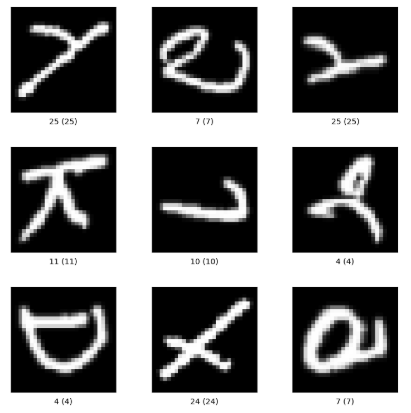
\includegraphics[width=0.5\textwidth]{emnist_letters.png}
\caption{A sample of the EMNIST Letter dataset.}
\label{FigUH}
\end{figure}

\subsection{Accuracy Calculation}
\label{sec:AccuracyCalculation}
To calculate the accuracy of the model, the categorical accuracy of the
model will be used. To perform the calculation, the \href{https://github.com/keras-team/keras/blob/c2e36f369b411ad1d0a40ac096fe35f73b9dffd3/keras/metrics.py}{categorical\_accuracy} function
from the Keras library will be used. This is the mathematical equivalent to the
accuracy calculation described in the OAR project's VnV Plan \citep{OARVnVPlan}.

% \subsection{Symbolic Parameters}

% The definition of the test cases will call for SYMBOLIC\_CONSTANTS.
% Their values are defined in this section for easy maintenance.

% \subsection{Usability Survey Questions?}

% \wss{This is a section that would be appropriate for some projects.}

\end{document}